% !TeX program = pdfLaTeX
\documentclass[journal]{vgtc}\usepackage{graphicx, color}
%% maxwidth is the original width if it is less than linewidth
%% otherwise use linewidth (to make sure the graphics do not exceed the margin)
\makeatletter
\def\maxwidth{ %
  \ifdim\Gin@nat@width>\linewidth
    \linewidth
  \else
    \Gin@nat@width
  \fi
}
\makeatother

\IfFileExists{upquote.sty}{\usepackage{upquote}}{}
\definecolor{fgcolor}{rgb}{0.2, 0.2, 0.2}
\newcommand{\hlnumber}[1]{\textcolor[rgb]{0,0,0}{#1}}%
\newcommand{\hlfunctioncall}[1]{\textcolor[rgb]{0.501960784313725,0,0.329411764705882}{\textbf{#1}}}%
\newcommand{\hlstring}[1]{\textcolor[rgb]{0.6,0.6,1}{#1}}%
\newcommand{\hlkeyword}[1]{\textcolor[rgb]{0,0,0}{\textbf{#1}}}%
\newcommand{\hlargument}[1]{\textcolor[rgb]{0.690196078431373,0.250980392156863,0.0196078431372549}{#1}}%
\newcommand{\hlcomment}[1]{\textcolor[rgb]{0.180392156862745,0.6,0.341176470588235}{#1}}%
\newcommand{\hlroxygencomment}[1]{\textcolor[rgb]{0.43921568627451,0.47843137254902,0.701960784313725}{#1}}%
\newcommand{\hlformalargs}[1]{\textcolor[rgb]{0.690196078431373,0.250980392156863,0.0196078431372549}{#1}}%
\newcommand{\hleqformalargs}[1]{\textcolor[rgb]{0.690196078431373,0.250980392156863,0.0196078431372549}{#1}}%
\newcommand{\hlassignement}[1]{\textcolor[rgb]{0,0,0}{\textbf{#1}}}%
\newcommand{\hlpackage}[1]{\textcolor[rgb]{0.588235294117647,0.709803921568627,0.145098039215686}{#1}}%
\newcommand{\hlslot}[1]{\textit{#1}}%
\newcommand{\hlsymbol}[1]{\textcolor[rgb]{0,0,0}{#1}}%
\newcommand{\hlprompt}[1]{\textcolor[rgb]{0.2,0.2,0.2}{#1}}%

\usepackage{framed}
\makeatletter
\newenvironment{kframe}{%
 \def\at@end@of@kframe{}%
 \ifinner\ifhmode%
  \def\at@end@of@kframe{\end{minipage}}%
  \begin{minipage}{\columnwidth}%
 \fi\fi%
 \def\FrameCommand##1{\hskip\@totalleftmargin \hskip-\fboxsep
 \colorbox{shadecolor}{##1}\hskip-\fboxsep
     % There is no \\@totalrightmargin, so:
     \hskip-\linewidth \hskip-\@totalleftmargin \hskip\columnwidth}%
 \MakeFramed {\advance\hsize-\width
   \@totalleftmargin\z@ \linewidth\hsize
   \@setminipage}}%
 {\par\unskip\endMakeFramed%
 \at@end@of@kframe}
\makeatother

\definecolor{shadecolor}{rgb}{.97, .97, .97}
\definecolor{messagecolor}{rgb}{0, 0, 0}
\definecolor{warningcolor}{rgb}{1, 0, 1}
\definecolor{errorcolor}{rgb}{1, 0, 0}
\newenvironment{knitrout}{}{} % an empty environment to be redefined in TeX

\usepackage{alltt}                % final (journal style)
%\documentclass[review,journal]{vgtc}         % review (journal style)
% \documentclass[widereview]{vgtc}             % wide-spaced review
%\documentclass[preprint,journal]{vgtc}       % preprint (journal style)
%\documentclass[electronic,journal]{vgtc}     % electronic version, journal

\usepackage{mathptmx}
\usepackage{graphicx}
\usepackage{times}

\usepackage{natbib}
\usepackage{fullpage}
\usepackage{color}
\usepackage[dvipsnames,svgnames]{xcolor}
\usepackage[bookmarks,backref=true,linkcolor=black]{hyperref} %,colorlinks
\hypersetup{
  pdfauthor = {},
  pdftitle = {},
  pdfsubject = {},
  pdfkeywords = {},
  colorlinks=true,
  linkcolor= black,
  citecolor= black,
  pageanchor=true,
  urlcolor = black,
  plainpages = false,
  linktocpage
}
\usepackage{wrapfig,float}
% \usepackage{caption}
\usepackage{subcaption}
\usepackage{amssymb}
\usepackage{amsmath}
\usepackage{url}
\usepackage{ulem}
\usepackage[section]{placeins}

% test change
% help with editing and coauthoring
\usepackage[colorinlistoftodos]{todonotes}

\newcommand{\hh}[1]{{\color{orange} #1}}

\graphicspath{{figure/}}
\renewcommand{\floatpagefraction}{.99}

\newcommand{\done}[2][inline]{\todo[color=SpringGreen, #1]{#2}}  % for todos that have been seen and dealt with
\newcommand{\newdo}[1]{\todo[inline, color=Plum]{#1}} % new to do item
\newcommand{\comment}[2][inline]{\todo[color=SkyBlue, #1]{#2}} % for comments that may not be "to-do"s
\newcommand{\newtext}[1]{\todo[inline, color=White]{ \color{OliveGreen}{#1}}} % new text - not necessarily something to be done

\begin{knitrout}
\definecolor{shadecolor}{rgb}{0.969, 0.969, 0.969}\color{fgcolor}\begin{kframe}


{\ttfamily\noindent\color{warningcolor}{\#\# Warning: Removed 150 rows containing missing values (geom\_path).}}

{\ttfamily\noindent\color{warningcolor}{\#\# Warning: Walker's alias method used: results are different from R < 2.2.0}}\end{kframe}
\end{knitrout}


%% If you are submitting a paper to a conference for review with a double
%% blind reviewing process, please replace the value ``0'' below with your
%% OnlineID. Otherwise, you may safely leave it at ``0''.
\onlineid{0}

%% declare the category of your paper, only shown in review mode
\vgtccategory{Research}

%% allow for this line if you want the electronic option to work properly
\vgtcinsertpkg

%% In preprint mode you may define your own headline.
%\preprinttext{To appear in an IEEE VGTC sponsored conference.}

%% Paper title.

\title{The curse of three dimensions: Why your brain is lying to you}
\author{Susan VanderPlas\thanks{e-mail: srvanderplas@gmail.com}\\ %
        \scriptsize Iowa State University %
\and Heike Hofmann\thanks{e-mail:hofmann@iastate.edu}\\ %
        \scriptsize Iowa State University %
\and Di Cook\thanks{e-mail:dicook@iastate.edu}\\ %
        \scriptsize Iowa State University %}
}
        
\abstract{One of the basic principles of visual graphics is that the graphic should accurately reflect the data.
Tufte's lie factor~\citep{tufte} was created with the idea that graphs that do not represent the underlying data accurately should be avoided. In this paper, we examine a second level of graph distortion that occurs during the perceptual process.
 The human visual system is largely optimized for perception of three dimensions. Generally, the brain processes potential  ambiguities in the rendering as the most-common three-dimensional object. This can lead to visual distortions, such as occur with the Necker figure or in the M\"uller-Lyer illusion.
We discuss the underlying psychological mechanisms for the distortions, examine the effect these distortions have on  judgments, and consider the implications for graph design. Using the sine illusion as a case study, we quantify the effects of the distortion that create a ``perceptual lie factor" for the sine illusion.}

 %% Uncomment below to include a teaser figure.
 %% Note: No figures other than the optional teaser are permitted on title page.
 %\centering
 %
\includegraphics[width=16cm]{CypressView.eps}
 %\caption{In the Clouds: Vancouver from Cypress Mountain}
 %} 
 
\begin{document}

\maketitle
% \section*{Outline}
% \begin{enumerate}
% \item Introduction - Lie Factor, Psychological Distortions, etc.
% \item Underlying Psychology - Why 3d perception is a curse. Muller Lyer, Ames room, etc. Necessity of quantifying the size of these effects on graphs to determine the psychological ``lie factor".
% \item Case Study - Sine Illusion
% \item Conclusions
% \end{enumerate}

\firstsection{Introduction}
One of the basic principles of visual graphics is that the graphic should accurately reflect the data. Tufte's ``Lie Factor", for instance, is calculated based on the ratio of the effect size shown in the graphic to the effect size in the data~\citep{tufte}. If there is a systematic difference, the lie factor will be notably different from 1 (values between .95 and 1.05 are typically acceptable). The implications behind Tufte's lie factor are somewhat ambiguous, however: Is the goal to make the graph on paper accurately represent the numbers used to generate that graph? Or is the goal to accurately convey the information presented in the graph to the reader? While in many cases these two goals can be achieved simultaneously, there are many instances in which human perception produces a psychological distortion that  interferes with the interpretation of graphics that are technically true to the numerical data. In this paper, we examine several situations in which very low-level human perceptual processes interfere with making accurate judgements from displays.
%that are true to the data. 

\section{The Curse of Three Dimensions}
The human visual system is largely optimized for perception of three dimensions. Biologically, binocular vision ensures that we have the necessary information to construct a three-dimensional world, but even in the absence of binocular information the brain uses numerous heuristics to parse otherwise ambiguous two-dimensional retinal images into meaningful three-dimensional mental representations of the world. Predictably, however, these heuristics are not without drawbacks; the same two-dimensional neural representation might correspond to multiple three-dimensional objects, as in the Necker Cube shown in Figure~\ref{fig:Necker}, while on the other hand, the same three-dimensional object often has infinitely many two-dimensional representations, for instance, when viewed from different angles. 
\begin{figure}[H]
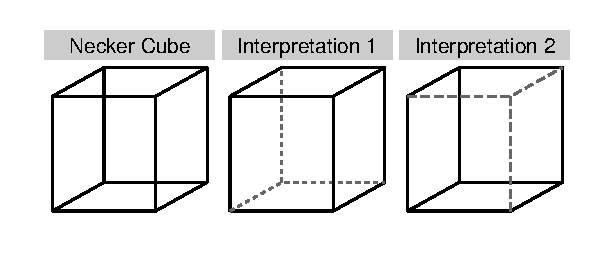
\includegraphics[keepaspectratio=TRUE,width=\linewidth]{figure/fig-neckercube}
\caption{The Necker Cube is a so-called ``ambiguous object" because two different transparent objects could produce the same perceptual experience. Commonly, perception seems to transition instantaneously from one possible mental representation to the other.}\label{fig:Necker}
\end{figure}
In the case of the Necker cube, the two different figures are equally salient, and thus the brain does not prefer one interpretation over the other and instead continuously switches between interpretations. In many cases, however, experience with the real world  informs the choice between multiple possible three-dimensional objects which form the same two-dimensional picture. This indicates that processing occurs ``top down" in that our previous experience influences our current perceptions. Without this top-down influence, the brain would not be able to map the picture back to the original three-dimensional object. One of the most well studied examples of the influence of top-down processing is the M\"uller-Lyer illusion, shown in Figure~\ref{fig:mullerlyer}

\begin{figure}[h!t]\centering
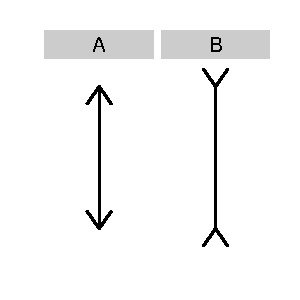
\includegraphics[keepaspectratio=TRUE]{figure/fig-mullerlyer}
\caption{The M\"uller-Lyer illusion. The central segment of Figure A is perceived as shorter than the central segment  of Figure B, even though the two are actually the same length.}\label{fig:mullerlyer}
\end{figure}

The M\"uller-Lyer illusion occurs because the brain interprets the ambiguous lines as a common three-dimensional object: corners of a room: Figure~\ref{fig:mullerlyer}A occurs when viewing the outside corner of a rectangular prism, Figure~\ref{fig:mullerlyer}B occurs when viewing the prism from the inside.  In regions which do not commonly have rectangular buildings, the illusion is significantly less pervasive~\citep{mullerlyerafrica}. Figure~\ref{fig:mullerlyerreal} demonstrates the real-world experience that would lead to the M\"uller-Lyer effect. This real-world experience carries with it an inferred perspective - when the arrows point inward, the object is typically closer than when the arrows point outward, which causes the brain to interpret the outward-pointing figure as larger, even though the retinal size is identical for the two objects. This inferred ``depth cue"~\citep{gregory} is reasonably consistent across individuals. A similar effect can also be found in the Necker Cube - whichever face appears to be furthest away also seems larger, even though any two parallel faces are equally sized in the image. The advantages of this approach in the real world are considerable~\citep{gregory}, as pictures of real objects are seldom ambiguous and this strategy allow for high performance with limited neural bandwidth - Figure~\ref{fig:mullerlyerreal} shows not only the real-world context, but that the perspective cues that contribute to the illusion allow for an accurate neural representation of the actual object. 

\begin{figure}[h!t]\centering
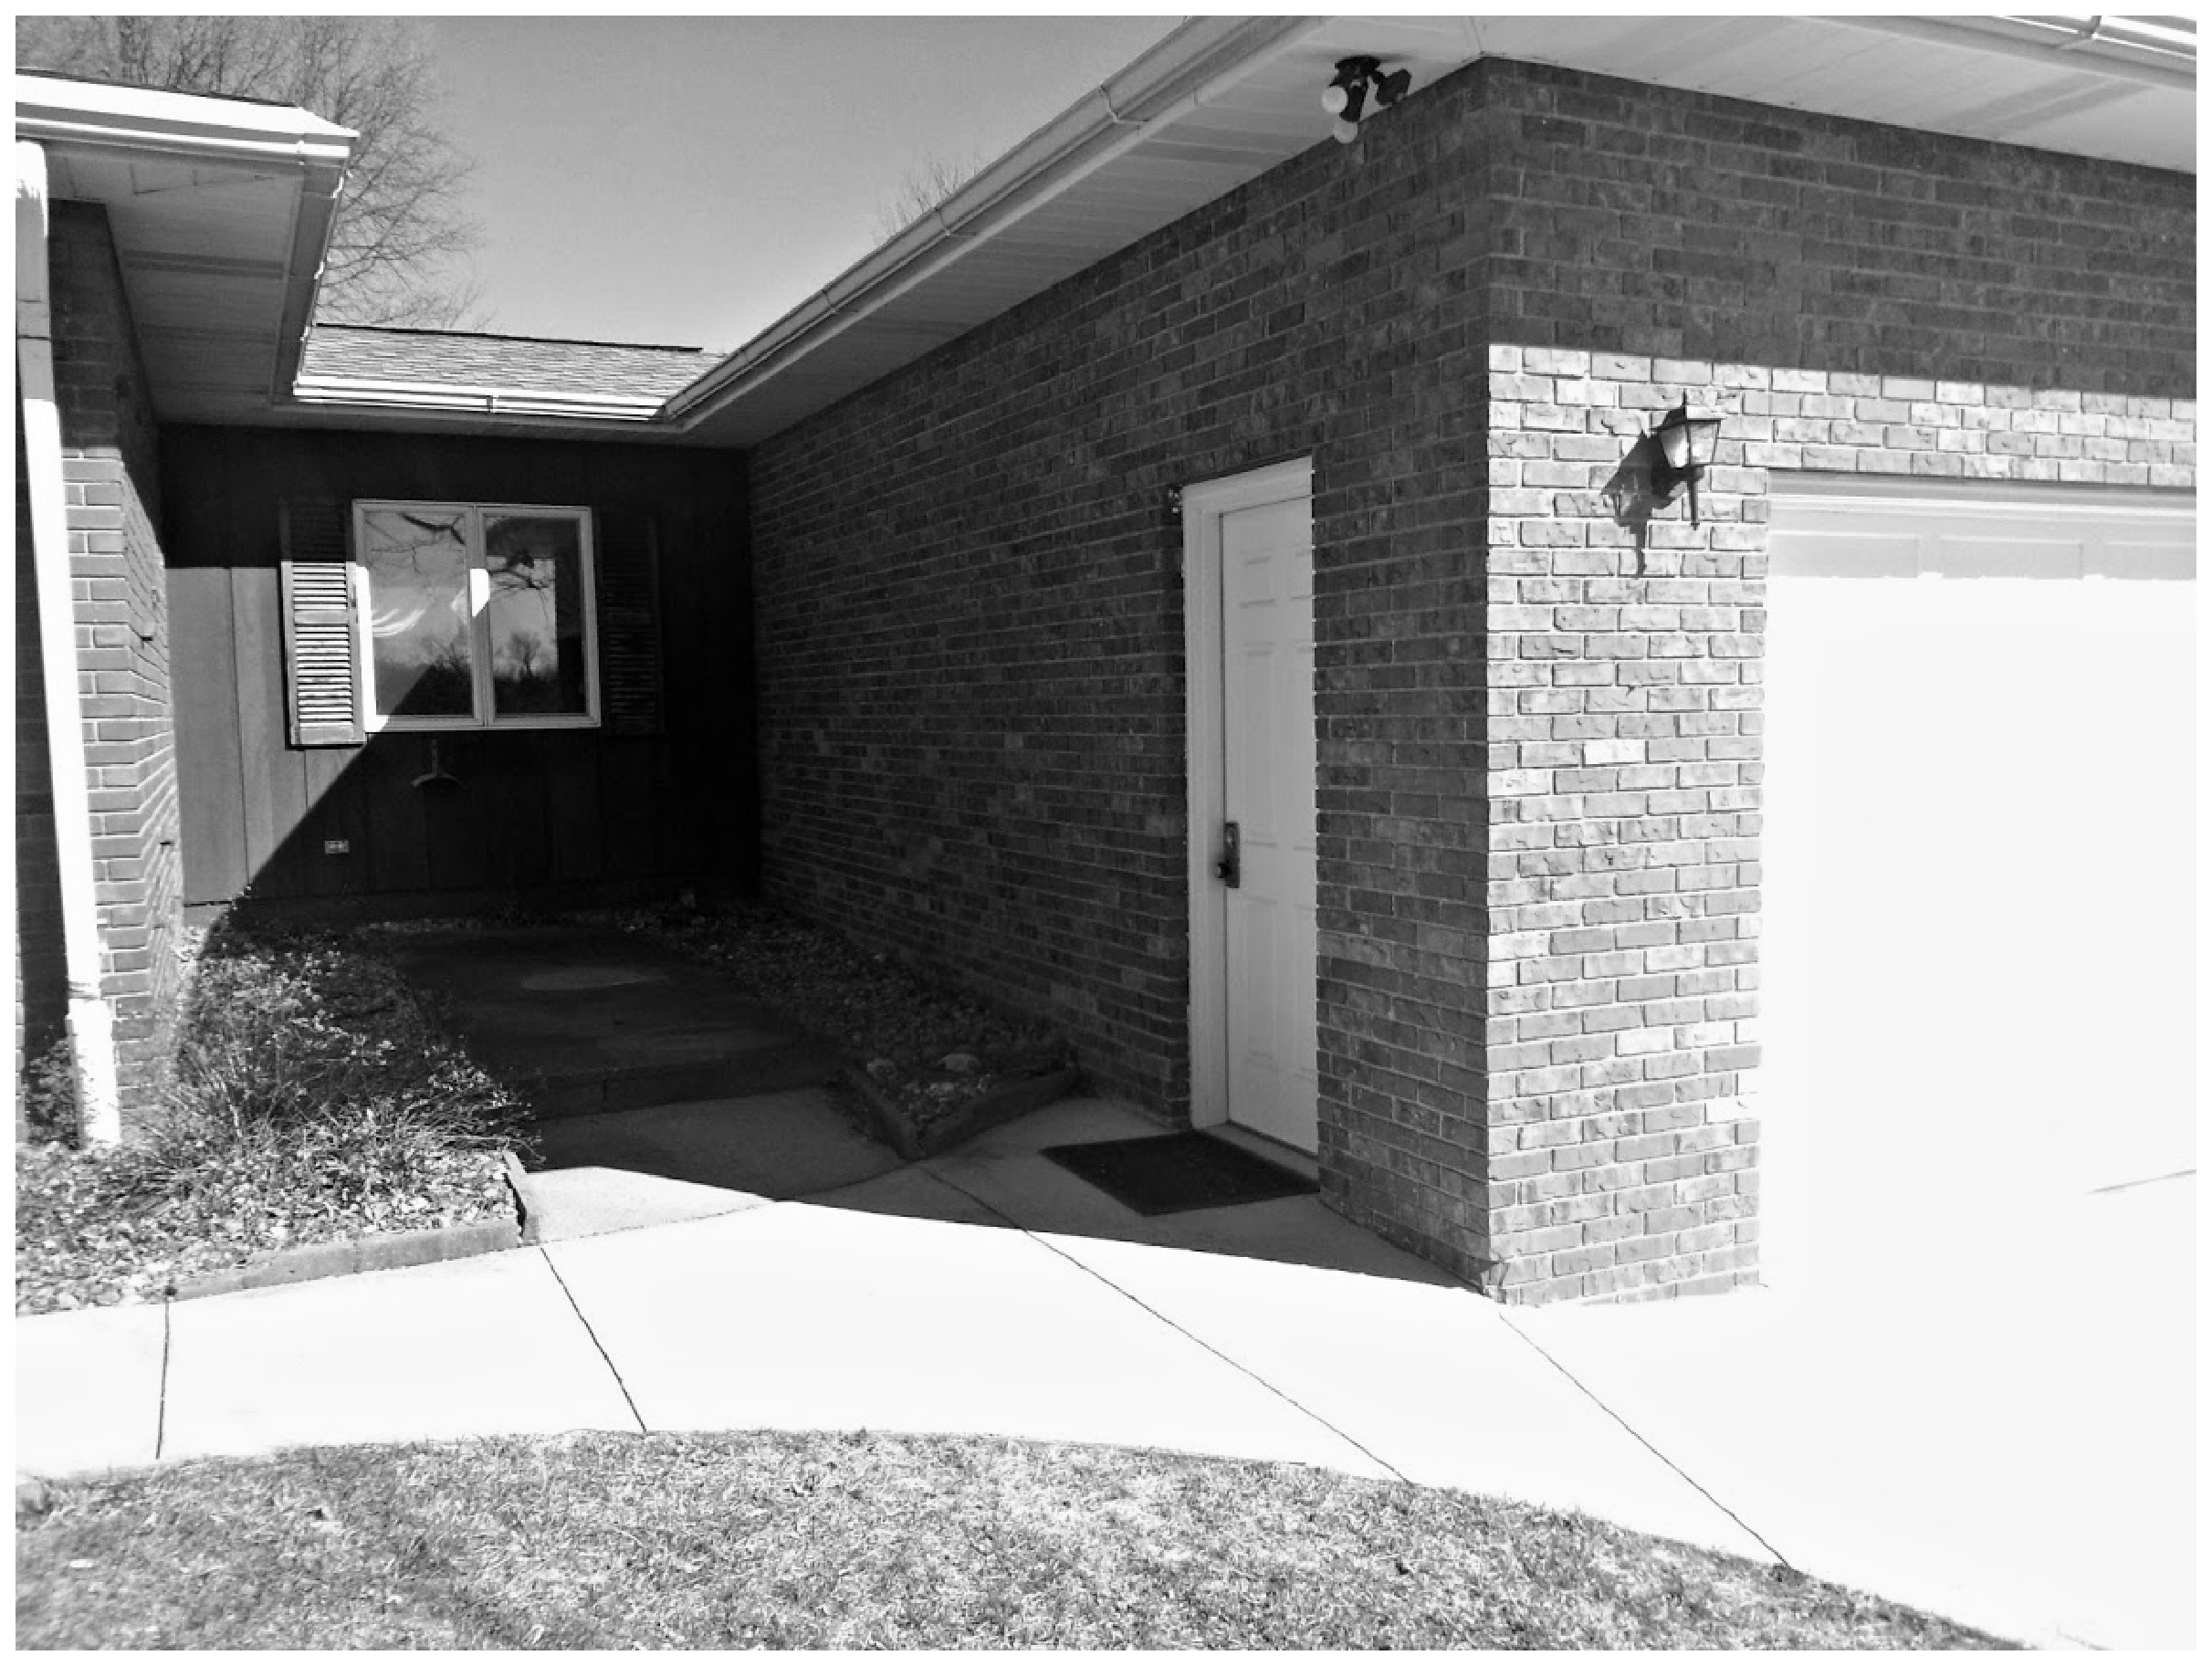
\includegraphics[keepaspectratio=TRUE,width=\linewidth]{images/mullerlyerhouse}
\caption{Real-world context that gives rise to the M\"uller-Lyer illusion}\label{fig:mullerlyerreal}
\end{figure}

\section{Three Dimensional Context of the Sine Illusion}
While the classic M\"uller-Lyer illusion is seldom a factor in statistical graphics, there are other illusions caused by the same mechanism: the brain interprets a two-dimensional stimulus in the context of three-dimensional objects, causing a distortion in the mental representation of the original stimulus. The sine illusion (also known as the line width illusion) is one example of this phenomenon which occurs frequently in statistical graphics. Like the M\"uller-Lyer illusion, it is pervasive and very difficult to ``un-see" or mentally correct. Figure~\ref{fig:sineillusion} shows the sine illusion in its original form, and Figure~\ref{fig:playfair} shows the same illusion in one of the charts from Playfair's Statistical Atlas~\citep{playfair}.
\begin{figure}[h!t]\centering
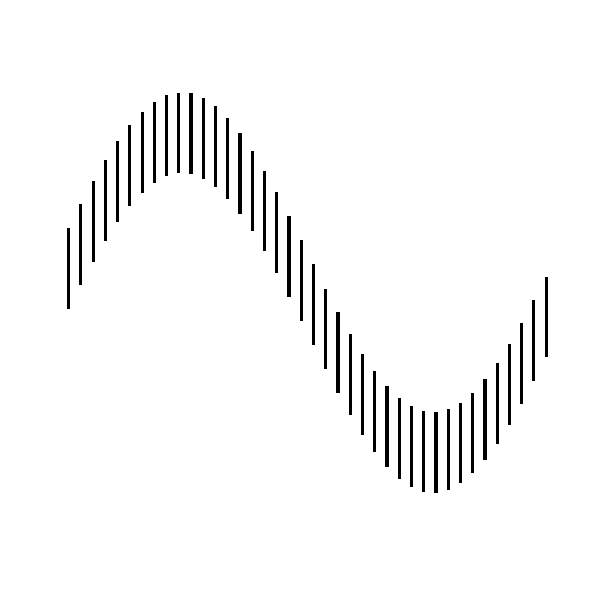
\includegraphics[keepaspectratio=TRUE,width=\linewidth]{figure/fig-sinedemo1}
\caption{The classic sine illusion. Each vertical line has the same length, though the lines at the peak and trough of the curve appear longer.}\label{fig:sineillusion}
\end{figure}

\begin{figure}[h!t]\centering
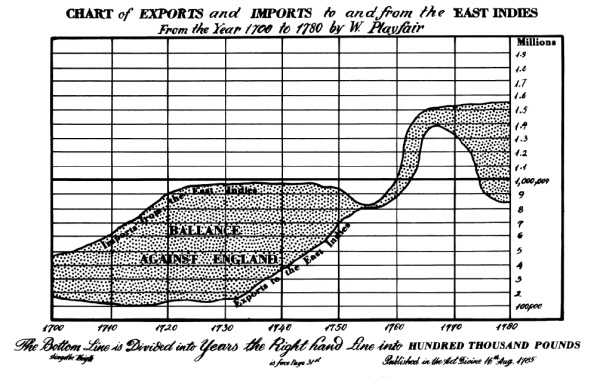
\includegraphics[keepaspectratio=TRUE,width=\linewidth]{images/PlayfairExportImports}
\caption{The sine illusion in Playfair's graph of trade between the East Indies and England, 1700-1780. The trade balance in 1763 does not appear to be the same size as that in 1745, though the vertical distance is approximately the same.}\label{fig:playfair}
\end{figure}
Cleveland and McGill
\citep{cleveland:1984} determined that comparison of vertical distances is inaccurate, as ``the brain wants to judge minimum distance between the curves in different regions, and not vertical distance". While they do not explain a reason for this tendency, introspection does readily confirm their explanation: we judge the distance between two curves based on the shortest distance between them, which geometrically is the distance along the line perpendicular to the tangent line of the curve. Day \& Stecher~\citep{day:1991} suggest that the sine illusion is similar in principle to the M\"uller-Lyer illusion, attributing it to the perceptual compromise between the vertical extent and the overall dimensions of the figure. The sine illusion is similar to the  M\"uller-Lyer illusion in another way, as well - there are three-dimensional analogues of the two-dimensional image that may influence the perceptual context. One of these contexts is shown in Figure~\ref{fig:sineillusion3d}, generated from the same function shown in the two-dimensional analogue, Figure~\ref{fig:sineillusion}, but with the length projected onto a third dimension. While the images do not match exactly, the similarities are striking. Additionally, the tendency to judge vertical distance using the extant width noted in Cleveland et al~\citep{cleveland:1985} corresponds to the measurement of depth in the three-dimensional image. One main difference between the three dimensional image shown in Figure~\ref{fig:sineillusion3d} and the original image is that the lines connecting the top and bottom sections of the curve are slightly angled in the three-dimensional version; this is due to the perspective projection used to create the image and the corresponding angles of rotation chosen such that the entire surface is visible. 

\begin{figure}[h!t]\centering
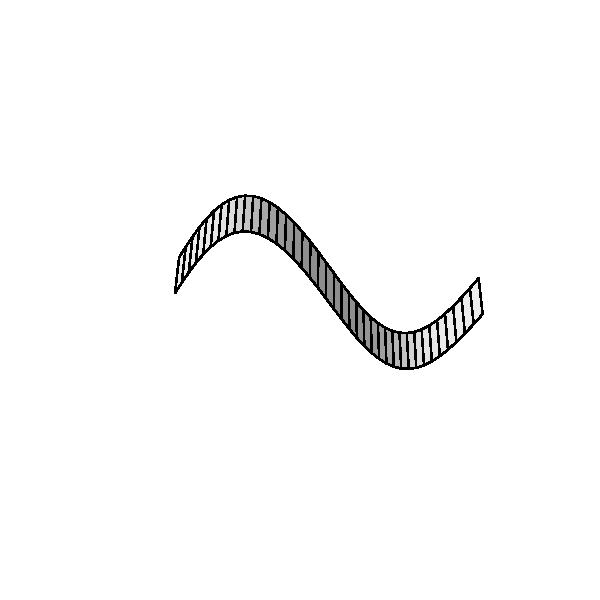
\includegraphics[keepaspectratio=TRUE,width=\linewidth, trim=0in 1.5in 0in 1.5in]{figure/fig-sinedemo2}
\caption{Three dimensional context for the sine illusion.}\label{fig:sineillusion3d}
\end{figure}

One difference between the sine illusion and the M\"uller-Lyer illusion that may influence the tendency to see a three-dimensional ``ribbon" instead of the two-dimensional sine curve is that the vertical lines in the sine illusion are ambiguously oriented - there is an entire plane of possible three-dimensional reconstructions for each line, and each possible rotation leads to a line of different length. It is this facet of the image that we believe partially contributes to the ambiguity of the image, though it is not a necessary feature for the illusion to persist, as the illusion also can be found in scatterplots and in ``ribbon plots" such as Figure~\ref{fig:playfair}. 


\begin{figure}[h!t]\centering
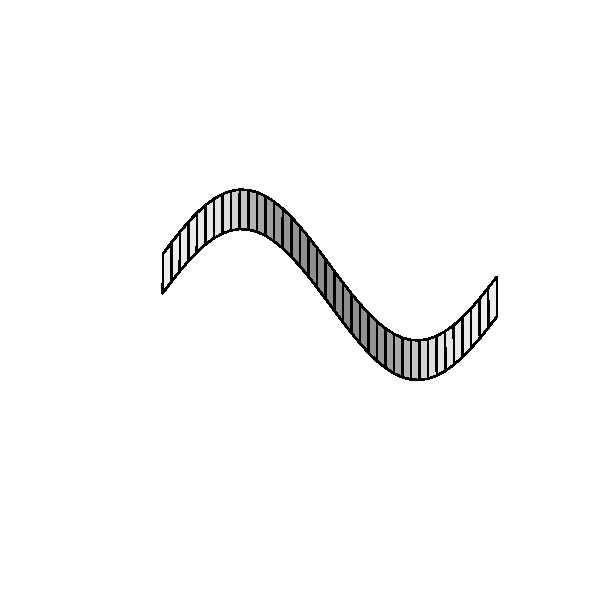
\includegraphics[keepaspectratio=TRUE,width=\linewidth, trim=0in 1.5in 0in 1.5in]{figure/fig-sinedemo3}
\caption{Three dimensional context for the sine illusion, with a weaker perspective transformation.}\label{fig:sineillusion3dmagic}
\end{figure}


Further, the three-dimensional reconstruction of the illusion converges on the actual picture as the vanishing point moves further away from the viewer and the 3d projection decreases in strength. Figure~\ref{fig:sineillusion3dmagic} shows a weaker 3-dimensional projection that is much closer to Figure~\ref{fig:sineillusion}, however, the three-dimensional contextual information provided by the shading removes much of the illusion's distortions. This, too, is similar to the Muller-Lyer illusion - Figure~\ref{fig:mullerlyerreal} is not at all ambiguous - the contextual depth information provided by the rest of the surface of the house is sufficient to remove the illusion that the closer corner is in fact larger due to the perspective.

The psychological mechanisms which force three-dimensional context onto two-dimensional stimuli are useful adaptations to a three-dimensional world~\citep{gregory}, but they do have disadvantages. In order to estimate the psychological lie factor that occurs due to this illusion, we assessed the strength of the illusion experimentally. 

\section{Experimental Determination of the Size of the Psychological Lie Factor for the Sine Illusion}
\subsection{Study Setup}
In order to determine the amount of the psychological distortion, participants were presented with different sheets of sets of six graphs each, similar to Figure~\ref{fig:sinestimuli}. These sets of charts were constructed such that line lengths along a curve were varied to different degrees to counteract the illusion. Figure~\ref{fig:sinestimulinotrend} shows the amount of line correction used in each of the sub-plots above. Participants were asked  to answer the question: "In which graph is the size of the curve most consistent?". 
The phrasing `size of the curve' was chosen deliberately so as not to bias participants to explicitly measure line lengths. 

The amount of correction in each sub-plot was chosen such that each sheet contained one uncorrected curve together with a selection of curves corrected to various degrees using correction factors determined previously in an internal pilot study. In the sine curve, the correction factor we use for extending the length of the line segment at loctaion $x$ is given as
\[
w \cdot \cos x,
\]
where $w$ is varied between 0 (for no correction) and 1.5 (very strong correction). From the previous pilot study, we suspected values around $w = 0.8$ to be promising. This led to twelve sheets with correction factors as shown in table~\ref{tab:w}. The difficulty level of each of the sheets was determined by the similarity of the six plots shown.

\begin{figure*}
\center
\begin{subfigure}[b]{.9\linewidth}\centering
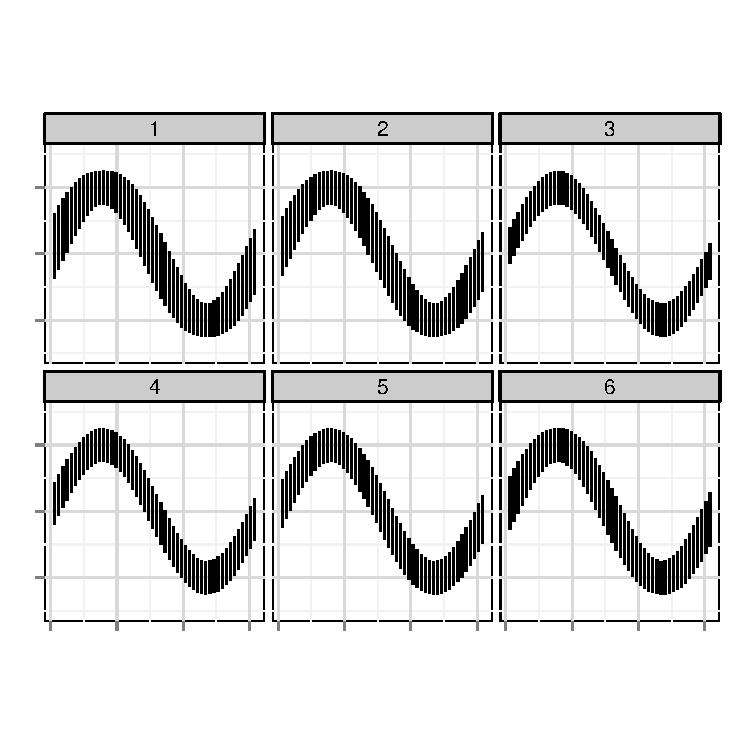
\includegraphics[width=.9\linewidth]{figure/fig-stimulicorrectionsize1}
\caption{One of the graphs presented to participants through Amazon Mechanical Turk.}\label{fig:sinestimuli}
\end{subfigure}
\begin{subfigure}[b]{.9\linewidth}\centering
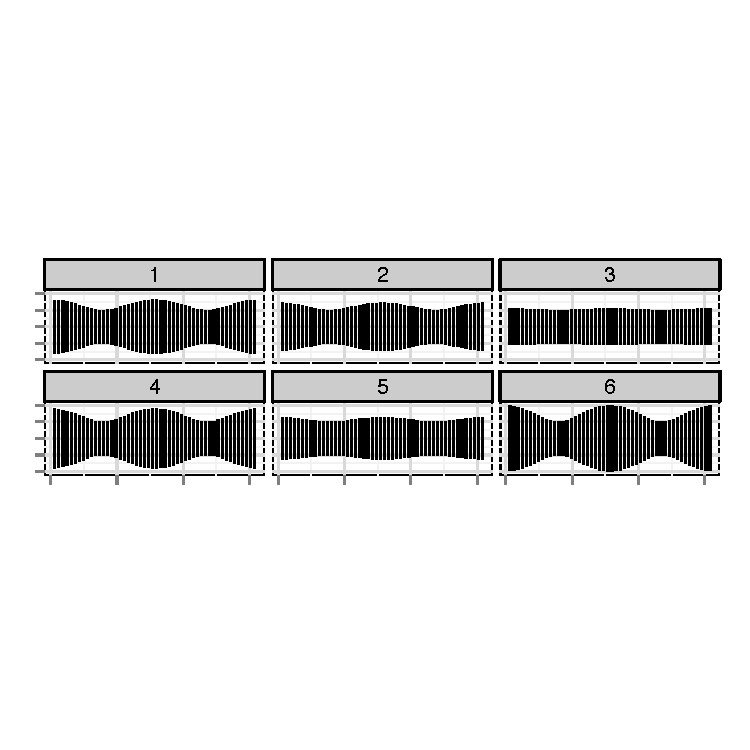
\includegraphics[width=.8125\linewidth]{images/fig-stimulicorrectionsize2}
\caption{Line lengths (without the trend) for Figure~\ref{fig:sinestimuli}.}\label{fig:sinestimulinotrend}
\end{subfigure}
\caption{Stimuli similar to (a) were shown to participants, while (b) shows the corresponding differences in line lengths.}
\end{figure*}
% latex table generated in R 2.15.1 by xtable 1.7-0 package
% Sun Mar 31 12:08:30 2013
\begin{table}[ht]
\centering
\begin{tabular}{rrrrrrrr}
  \hline
  & \multicolumn{5}{c}{sub-plot}\\\cline{2-7}\\ [-1.75ex]
set \vphantom{hp}& 1 & 2 & 3 & 4 & 5 & 6 & difficulty\\ 
  \hline
1 & 0.00 & 0.20 & 0.40 & 0.80 & 1.25 & 1.40 & test\\ 
  2 & 0.00 & 0.15 & 0.35 & 0.80 & 1.20 & 1.40 & test\\ 
  3 & 0.00 & 0.20 & 0.40 & 0.60 & 0.80 & 1.00 & 1 \\ 
  4 & 0.10 & 0.30 & 0.50 & 0.70 & 0.90 & 1.10 & 1 \\  
  5 & 0.00 & 0.50 & 0.70 & 0.80 & 0.90 & 1.00 & 2 \\ 
  6 & 0.00 & 0.45 & 0.65 & 0.75 & 0.85 & 1.00 & 2 \\ 
  7 & 0.40 & 0.70 & 0.80 & 0.90 & 1.00 & 1.30 & 3 \\  
  8 & 0.30 & 0.65 & 0.75 & 0.85 & 0.95 & 1.20 & 3 \\ 
  9 & 0.50 & 0.60 & 0.70 & 0.80 & 0.90 & 1.00 &  4 \\  
  10 & 0.55 & 0.65 & 0.75 & 0.85 & 0.95 & 1.00 & 4 \\ 
  11 & 0.60 & 0.70 & 0.75 & 0.85 & 0.90 & 1.00 & 5\\ 
  12 & 0.60 & 0.70 & 0.75 & 0.80 & 0.90 & 1.00 & 5\\ 
   \hline
\end{tabular}
\caption{\label{tab:w} Distortion factors used for the sine curve stimulus.}
\end{table}

Besides the sine wave two other curves were tested, as shown in figure~\ref{fig:stimuli}. Figure~\ref{fig:stimuli.a} shows an inverse function ($f(x) = 1/x$),  figure~\ref{fig:stimuli.b} shows line lengths along an exponential ($f(x) = \exp(a \cdot x)$). Note that for both figures the line lengths are kept constant.

\begin{figure}
\begin{subfigure}[b]{.49\linewidth}\centering
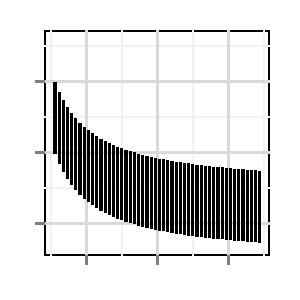
\includegraphics[width=\linewidth]{figure/fig-inverse}
\caption{inverse function.}\label{fig:stimuli.a}
\end{subfigure}
\begin{subfigure}[b]{.49\linewidth}\centering
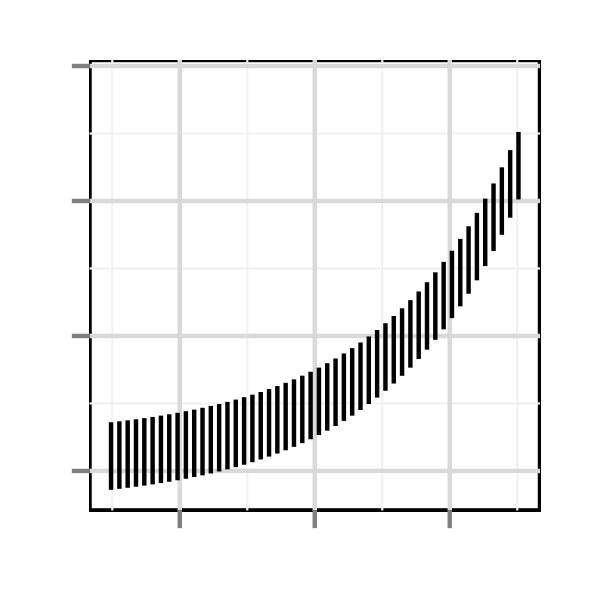
\includegraphics[width=\linewidth]{figure/fig-exponential}
\caption{exponential function.}\label{fig:stimuli.b}
\end{subfigure}
\caption{\label{fig:stimuli} Vertical line segments along two curves. Lengths of line segments are kept constant but appear to change  due to a strong contextual illusion.}
\end{figure}

Each participant was presented with eleven sets of graphs, consisting of five sheets of difficulty level 1 through 5 with the sine curve as stimuli, and another set of five sheets (also of difficulty levels 1 to 5) from either the exponential or the inverse curve, as well as a test chart. Plots were shown to participants in random order.
The test chart consists of a set of six sine curves with a very low level diffcilty level. We use the test chart to filter out participants providing us with spurious responses.

Additionally, participants were  asked to provide an estimate of their confidence in their answer, rated on a five point likert scale from low to high. 


% The 11 sets of graphs were broken down into 6 sets of sine plots as in Figure~\ref{fig:sinestimuli} and 5 sets of plots with either an inverse ($f(x) \propto 1/x$) or exponential ($f(x) \propto \exp(a*x)$) curve. Plots were shown to participants in random order, and were ranked by difficulty so that each participant received one plot of each of 5 levels of difficulty (as measured by the similarity of the 6 plots shown), plus a test sine plot that had the lowest difficulty for use in filtering out spurious responses. After the 11 plots required to receive payment through Amazon, participants could continue participating, and any subsequent plots were randomly selected from the 32 possible stimuli. 


\subsection{Demographics}
Participants for the study were recruited through the Amazon Turk web service. 
Each participant was asked to pick the curve with the minimal amount of length distortion from eleven sheets. Responses from 128 users at 123 unique IP addresses were collected. 
Some participants continued to provide feedback beyond the eleven required to receive payment through Amazon. For any subsequent responses we randomly selected one for each of the possible 32 stimuli.

In order to more accurately identify unique individuals, data were grouped by IP address rather than by user-entered identification code, as it is common for individuals to have multiple accounts and somewhat less likely for two Amazon Mechanical Turk participants to share the same IP address and complete the same study in the same reasonably short window. We treated responses from the  same IP addresses as additional responses from the same user.
%There were 123 unique IP addresses and 128 unique user ID values, so at most this decision affected 1/12 of the data. 

% The 11 sets of graphs were broken down into 6 sets of sine plots as in Figure~\ref{fig:sinestimuli} and 5 sets of plots with either an inverse ($f(x) \propto 1/x$) or exponential ($f(x) \propto \exp(a*x)$) curve. Plots were shown to participants in random order, and were ranked by difficulty so that each participant received one plot of each of 5 levels of difficulty (as measured by the similarity of the 6 plots shown), plus a test sine plot that had the lowest difficulty for use in filtering out spurious responses. After the 11 plots required to receive payment through Amazon, participants could continue participating, and any subsequent plots were randomly selected from the 32 possible stimuli. 



\subsection{Analysis}
\paragraph{Psychological ``Lie Factor"}
As the strength of the correction varies across the horizontal range of the curve, we  quantify the psychological distortion as the ratio of the maximum line length to the minimum line length for each plot $i$: $D^i = l_{max}/l_{min}$, and denote the chosen ratio as $D^\ast$. 
Without any correction, this factor is, as Tufte's lie-factor, equal to one, values above one indicate that at least in some areas of the curve line segments are extended.

% We compute this quantity for each plot in each set presented to the participant. The participant's choice therefore provides us with an estimate of what value of $D$ constitutes the most consistent line length (out of the set shown). As each set of 6 plots is not guaranteed to contain a plot with $w=0$, corresponding to constant length, choosing a plot with $D=1.4$ indicates more distortion if there is a $D_i=1$ also in the plot than if there is at minimum a $D=1.2$. This correction for the set of $D^\ast=\{D_1, ..., D_6\}$ that is available to choose from produces an estimate of the overall  psychological `lie factor' as 
% $$P=D^\ast/\min_{1\leq i \leq 6} D_i$$
% for each plot and each participant.
% 
% \hh{What is $D^\ast$ and why do we need to divide by the minimum of the other values of $D$? -- I fixed the math and elaborated a bit more. Since not every plot has a w=0 option, the lie factor of "what appears most constant" changes. I'm not sure that it's that big of a deal, to be honest... the outcome should be the same regardless, since both map back to $w$ linearly.}

%
By considering each participant's answers for the plot with the most consistent line length, we can obtain an estimate of the psychological distortion from the sine illusion on an individual level. 

This allows further investigation of the phenomenon.
In particular, similar values of $D$  across participants,   suggest the possibility of an underlying neural basis for the sine illusion, rather than a learned misperception. 

Each value of $w$ as defined in table~\ref{tab:w} corresponds  to a value of $D$ as defined above. 
We test for only a set of discrete values of $w$, which is reflected directly in the number of different values of $P$ we can observe. 
To counteract this discreteness, we employ a Bayesian approach to allow for a more precise estimation of the psychological lie-factor:

Plots used in the experiment have factors $D$ ranging between 0 and 3,  so we can use a normal data model for participant $i$ viewing plot $j$, with $D = D_{ij} \sim N(\theta, \sigma)$ and flat priors $\pi(\theta)=1/3\cdot I[0\leq\theta\leq 3]$ and $\pi(\sigma)=2$ for $\sigma\in[.1, .5]$. These ``prior distributions" $\pi(.)$ represent our expectations of the values of $\theta$ and $\sigma$ before the experiment; assigning them constant values indicates that we had little useable knowledge about the joint or marginal distributions of $\theta$ and $\sigma$ before the experiment was conducted. Using Bayesian estimation, we can then obtain posterior distributions for $\theta_i$ and $\theta$, the individual and overall mean lie factors. We are not particularly interested in the actual values of $\sigma$, but just use it as a tool to better estimate possible values for $\theta$.
An  advantage to using a normal distribution for $D$ and flat priors for $\theta$ and $\sigma$ is that the posterior distribution has a closed form that we can evaluate directly without resorting to Monte Carlo techniques.

\subsection{Results}
The overall posterior distribution of $\theta$ for each function is shown in Figure \ref{fig:overalldensity}. $\theta$ is reasonably similar for all three functions overall, and on an individual level, 
Figure~\ref{fig:indivdensity} shows the posterior density for $\theta_i$ for four of the participants who completed at least 6 trials in each category. 

\begin{figure}\centering
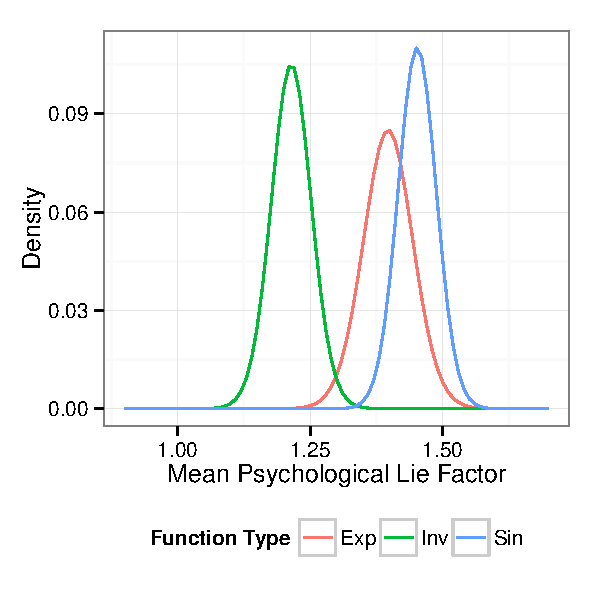
\includegraphics[width=\linewidth]{figure/fig-OverallMeans}
\caption{Posterior distributions for $\theta$ for each of the three stimuli types.}\label{fig:indivdensity}
\end{figure}

The posterior distributions for each function type are very similar, and the changing variance is at least in part due to the varying number of trials of each function type completed by each participant. This suggests that individuals have similar psychological distortions even for different functions. 


\begin{figure}\centering
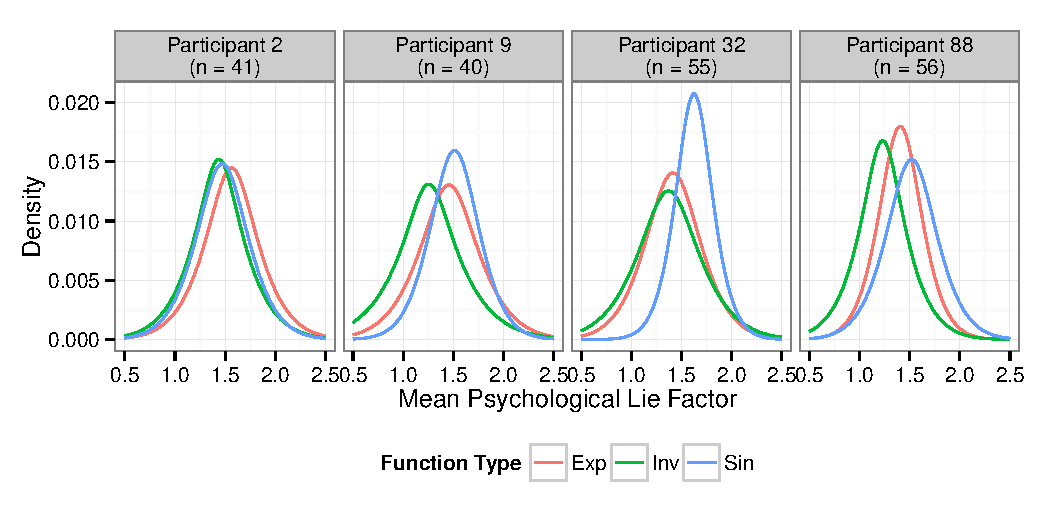
\includegraphics[width=\linewidth]{figure/fig-IndivMeanAllFcns}
\caption{Posterior distributions for $\theta_i$ for four of the participants who completed at least 6 trials of each of the three function types.}\label{fig:indivdensity}
\end{figure}

Credible intervals for $\theta_i$ as shown in Figure~\ref{fig:indivCIs} suggest that overall, the $\theta_i$ are similar across individuals. Very few of the intervals contain 1, indicating that there is significant distortion for most individuals, and the marked overlap of the intervals for each participant provides evidence towards a consistent magnitude of distortion and suggests there may be a common biological cause. 

\begin{figure}\centering
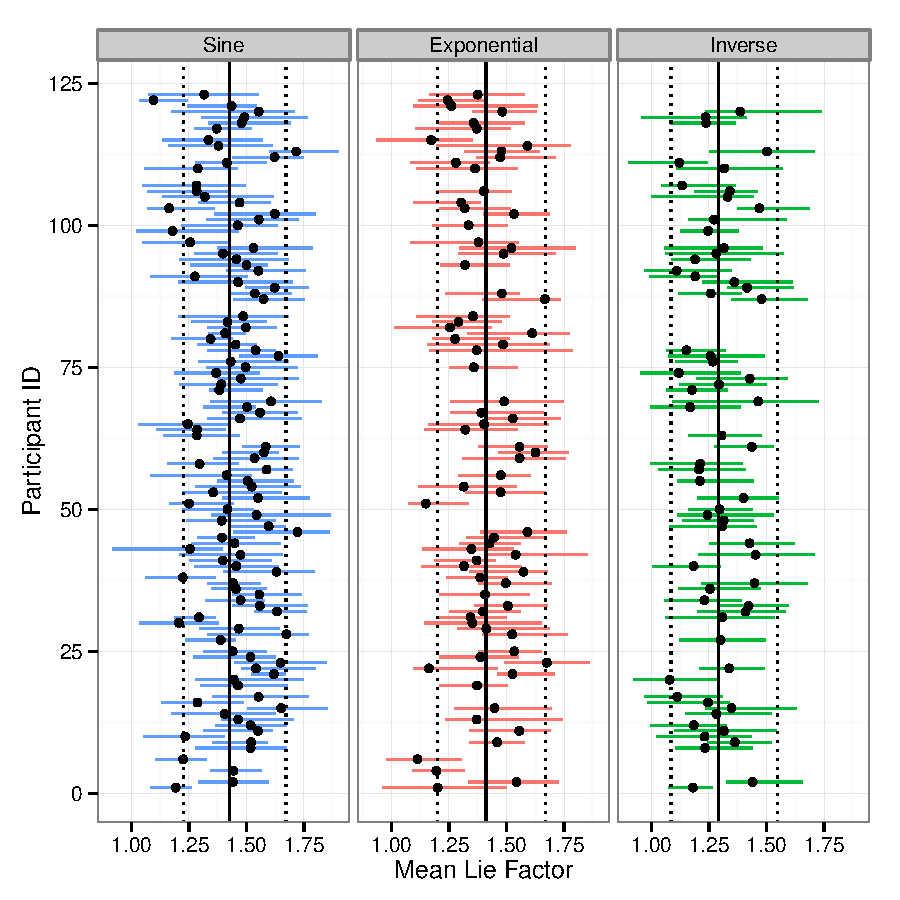
\includegraphics[width=\linewidth]{figure/fig-CIindivMean}
\caption{95\% credible intervals for each participant and stimulus type. Vertical lines indicate the median estimate of the overall $\theta$ with a 95\% credible interval.}\label{fig:indivCIs}
\end{figure}

The overall distribution of $\theta_i$ and $\theta$ for each stimulus type is shown in Figure~\ref{fig:overalldensity}. Estimates of $\hat\theta = E[\theta]$ for each function are 1.41, 1.3, and 1.44 respectively for exponential, inverse, and sine functions, suggesting a similar psychological distortion even for very different functions. Credible intervals can be found in Table \ref{tab:credibleintervalstable}.

\begin{table}\centering\begin{tabular}{ccc}
Function & 95\% Credible Interval for $\theta$ & Median\\\hline
Exp & (1.2016, 1.6707) & 1.4114\\
Inv & (1.0851, 1.5488) & 1.2932\\
Sin & (1.2267, 1.6718) & 1.4264\\
\hline
\end{tabular}
\caption{Credible intervals for the overall $\theta$ for exponential, inverse, and sine stimuli.}\label{tab:credibleintervalstable}\end{table}

\begin{figure}\centering
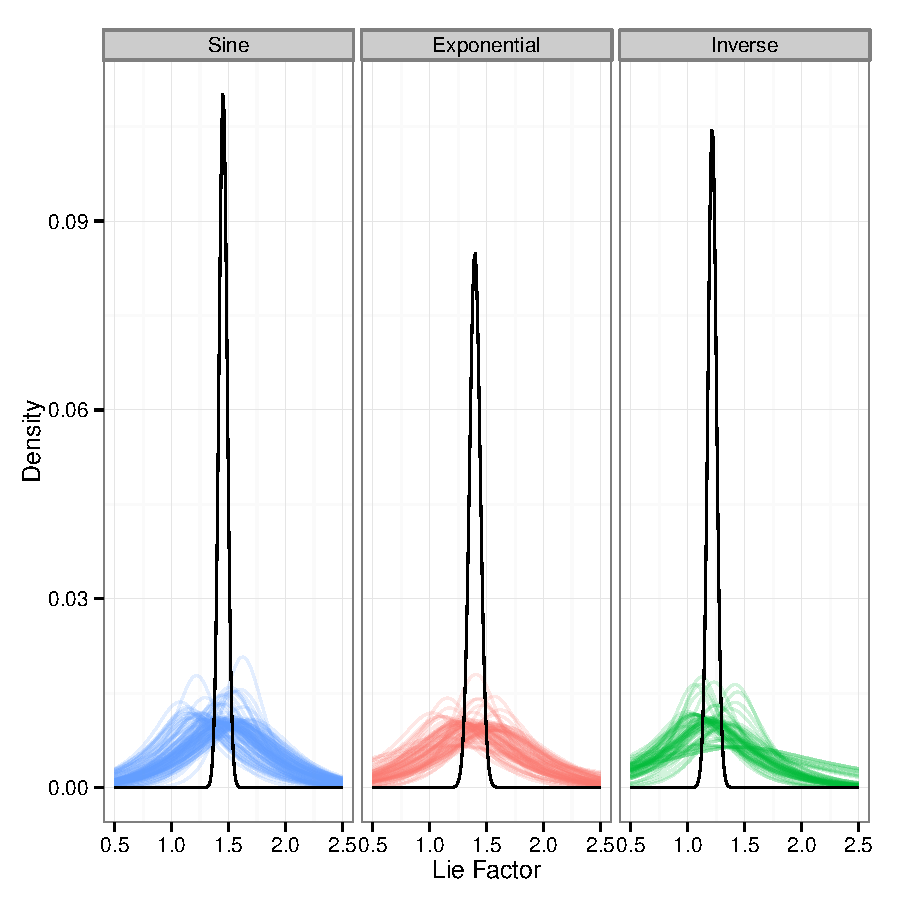
\includegraphics[width=\linewidth]{figure/fig-spaghettiIndivDists}
\caption{Estimated densities for $\theta_i$, shown in color, with the estimated overall density for $\theta$ shown in black. Individuals have extremely similar posterior distribution of $\theta_i$, and even different functions have similar $\hat\theta$, suggesting a common underlying mental distortion.}\label{fig:overalldensity}
\end{figure}

\subsection{Comparison of the Preferred Stimuli}
\begin{figure*}\centering
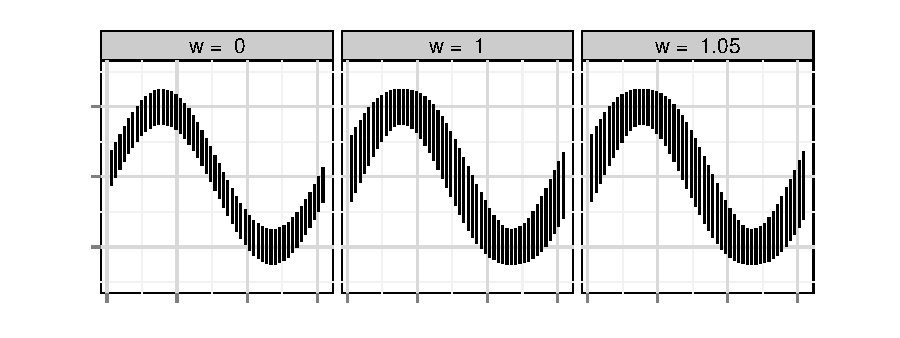
\includegraphics[width=\linewidth]{figure/fig-sineOptimalWeights}
\caption{Sine stimuli with uncorrected (w=0), optimally corrected (according to the mean value of $\theta$), and fully corrected (w=1)}\label{fig:sineCorrectionOptimal}
\end{figure*}
\begin{figure*}\centering
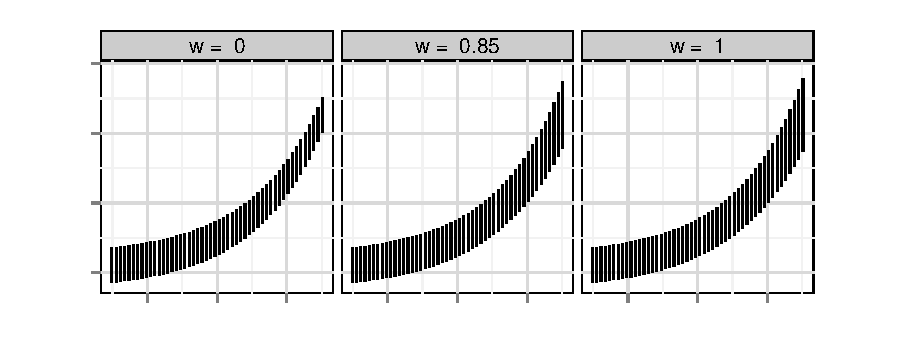
\includegraphics[width=\linewidth]{figure/fig-expOptimalWeights}
\caption{Exponential stimuli with uncorrected (w=0), optimally corrected (according to the mean value of $\theta$), and fully corrected (w=1)}\label{fig:expCorrectionOptimal}
\end{figure*}
\begin{figure*}\centering
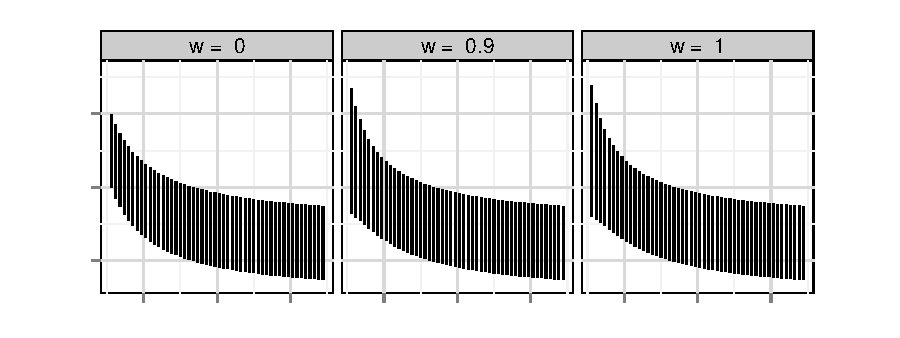
\includegraphics[width=\linewidth]{figure/fig-invOptimalWeights}
\caption{Exponential stimuli with uncorrected (w=0) , optimally corrected (according to the mean value of $\theta$), and fully corrected (w=1)}\label{fig:invCorrectionOptimal}
\end{figure*}

\section{Conclusions}
The sine illusion arises from misapplication of three-dimensional context to a two-dimensional stimulus which results in nearly unavoidable perceptual distortions that impact the inferences made from graphics. We have estimated that the illuson produces a distortion of about 140\%. This distortion occurs entirely between the retinal image and the mental representation of the object; it is not due to the chart, rather, it is an artifact of our perceptual system. As many graph types can induce this illusion (scatterplots, ribbon plots, parallel sets plots) we should be aware of its implications when drawing conclusions from graphical displays.

\clearpage
\bibliographystyle{plain}
\bibliography{references}











\end{document}
